\documentclass[11pt,a4paper]{ctexart}

\usepackage[a4paper,margin=2.4cm]{geometry}
\usepackage{graphicx}
\usepackage{booktabs}
\usepackage{amsmath,amssymb}
\usepackage{xcolor}
\usepackage{hyperref}
\usepackage{caption}
\usepackage{subcaption}
\usepackage{enumitem}
\usepackage{float}
\usepackage{array}

\hypersetup{colorlinks=true,linkcolor=blue!55!black,urlcolor=blue!55!black,citecolor=blue!55!black}

\captionsetup{font=small,labelfont=bf,labelsep=quad}
\setlist[itemize]{leftmargin=1.6em,itemsep=2pt,topsep=2pt}
\setlist[enumerate]{leftmargin=1.8em,itemsep=2pt,topsep=2pt}

% 全局图宽
\newcommand{\figwidefull}{0.92\linewidth}
\newcommand{\figwidehalf}{0.62\linewidth}
\newcommand{\figwidetall}{0.55\linewidth}

\title{\bfseries 基于生成对抗网络的人头图像生成与可控编辑}
\author{葛思如、杨骐宁}
\date{\today}

\begin{document}
\maketitle

\begin{abstract}
本文围绕生成对抗网络在人头图像生成任务上的实践展开。
我们首先实现并训练了一个深度卷积生成对抗网络作为基线，
在大规模对齐人脸数据上完成稳定训练，给出潜空间插值与
基于 Fr\'echet Inception Distance 与 Inception Score 的定量评估；
随后以预训练的高分辨率风格化生成器为主干，
复现了基于 CLIP 监督的潜空间映射器，
将自然语言描述对应的语义编辑能力注入到既有的解耦潜空间之中。
我们对训练动力学、损失项之间的权衡以及最终生成质量进行了
系统的定量与定性分析，并对常见的对抗训练病态如模式崩溃给出了
若干工程层面的缓解措施和实证观察。
\end{abstract}

\tableofcontents
\bigskip

%=================================================================
\section{引言}
%=================================================================
生成对抗网络通过生成器与判别器之间的极小极大博弈，
将简单先验分布映射到与真实样本一致的高维流形上，
是过去十年中最具影响力的隐式生成模型之一。
针对人头图像这一典型领域，已有研究沿两条路径快速发展：
一条是以全卷积结构、批归一化与对称转置卷积为骨架的卷积生成网络，
其结构简洁、训练成本可控，是理解对抗训练机理与常见病态的良好载体；
另一条则以风格调制和分层潜空间为核心，
通过将噪声先验映射到一个可解释、可解耦的中间空间，
取得了高分辨率人脸生成上的显著飞跃，并衍生出一系列
基于该中间空间的可控编辑方法。

本工作沿着上述两条路径分别构建了一套完整的训练与评估流水线。
基线侧实现了一个带谱归一化判别器与指数滑动平均生成器的卷积对抗网络，
在大规模对齐人脸数据上完成了八十轮的训练，
并对潜空间的两类典型插值方式进行了对比；
进阶侧采用预训练的风格化生成器，叠加一组按照分层语义划分的
潜空间映射器，以一组多样化的文本描述为条件分别训练，
从而获得在同一生成器之上「即插即用」的多种语义编辑能力。
在两条路径之间，我们以同一组指标度量样本质量与语义一致性，
形成了对比鲜明、互为补充的实验结果。

%=================================================================
\section{方法}
%=================================================================

\subsection{基础对抗生成网络}
\paragraph{生成器}
生成器以独立同分布的标准正态噪声 $z\in\mathbb R^{100}$ 为输入，
经过五层转置卷积逐级上采样，
每层卷积核为 $4\times 4$、步长为 $2$，配合批归一化与 ReLU 激活，
最终输出三通道、空间分辨率为 $64\times 64$ 的张量；
末层使用 Tanh 把像素值压缩到 $[-1,1]$，
与训练数据归一化范围保持一致。
\paragraph{判别器}
判别器结构与生成器对称，但每个卷积层均带有谱归一化约束，
以将每层算子的 Lipschitz 常数限制在 $1$ 以内，从而稳定对抗训练。
谱归一化与批归一化在实践中常常存在相互干扰的现象，
故判别器在加入谱归一化后我们移除了所有批归一化层，
并以 LeakyReLU 替代 ReLU，进一步缓和梯度饱和。
\paragraph{损失与优化}
生成器与判别器均以二分类交叉熵作为损失，
Adam 优化器的动量参数取经典的 $\beta_1=0.5,\beta_2=0.999$，
学习率取 $2\times 10^{-4}$，批大小为 $128$。
为进一步抑制判别器过早过自信，
我们在训练前期对判别器输入加入随训练进度线性退火的高斯噪声，
并对真实样本目标采用平滑标签。
\paragraph{滑动平均生成器}
我们以衰减系数 $\beta=0.999$ 维护一份生成器参数的指数滑动平均副本，
所有采样、插值与定量评估均统一使用滑动平均权重，
以平滑训练后期的振荡并提供更稳定的样本质量估计。

\subsection{潜空间插值}
为验证生成器学到的是连续而非离散的人脸流形，
我们对两个独立采样的噪声向量 $z_0,z_1$ 之间做两类插值。
线性插值定义为 $z_t=(1-t)z_0+tz_1$，实现简单但中段范数会向零收缩，
导致中间样本相对于真实先验偏离较远；
球面插值则沿着两点张成的二维平面上的大圆弧前进
\begin{equation}
z_t=\frac{\sin((1-t)\Omega)}{\sin\Omega}z_0+\frac{\sin(t\Omega)}{\sin\Omega}z_1,
\quad \Omega=\arccos\!\left(\tfrac{\langle z_0,z_1\rangle}{\|z_0\|\,\|z_1\|}\right),
\end{equation}
能在标准正态先验下保持范数不变，因此通常是更合适的默认选择。
我们在结果一节中同时给出两类路径的对比。

\subsection{评估指标}
我们采用 Fr\'echet Inception Distance 与 Inception Score 两项指标进行定量评估。
前者用预训练 Inception 网络的特征分布距离衡量生成分布与真实分布之间的接近程度，
后者衡量生成样本本身的清晰度与多样性。
评估时分别从真实数据集与生成器中采样足够数量的图像，
统一按训练阶段同样的预处理流程对齐到目标分辨率，
再交由公开评估工具完成度量。

\subsection{基于风格化生成器的可控编辑}
基础对抗生成网络在低分辨率上能够稳定生成可识别的人脸，
但在高频细节、身份保真与可控性上存在明显瓶颈。
为获得高分辨率与细粒度可控性，我们采用一类风格化生成器作为进阶骨干。
其核心思想是先把噪声经过一个映射网络变换为风格向量，
再以风格向量逐层调制各分辨率的合成路径。
经多层调制后，分层风格向量构成一个表达能力强、
语义解耦良好的中间潜空间，常被记为 $\mathcal W^+$。

\paragraph{分层潜空间映射器}
为将自然语言条件注入既有的解耦潜空间，我们引入一组
按层语义划分的轻量映射网络。
具体地，把 $\mathcal W^+$ 在层维度上划分为粗、中、细三段，
分别对应整体形状与姿态、五官与表情、颜色与纹理；
每段独立由一个四层等化线性结构组成的多层感知机
建模该段位移 $\Delta w$，整体输出
$\Delta w_+=[\Delta w_\mathrm{coarse};\Delta w_\mathrm{medium};\Delta w_\mathrm{fine}]$。
最终生成的图像由
\begin{equation}
\hat x = G(w_+ + \Delta w_+)
\end{equation}
得到，其中 $G$ 为冻结参数的预训练风格化生成器。
这一结构的优势在于：粗、中、细三段的解耦使得
不同语义层次上的编辑可以独立学习与开关，
也避免了一次性扰动整段 $\mathcal W^+$ 带来的不稳定。

\paragraph{文本条件下的损失函数}
给定一条文本描述 $t$，针对该描述独立训练一个映射器，
训练目标为如下三项的加权和
\begin{equation}
\mathcal L = \lambda_\mathrm{CLIP}\,\mathcal L_\mathrm{CLIP}\!\left(\hat x, t\right)
+ \lambda_\mathrm{ID}\,\mathcal L_\mathrm{ID}\!\left(\hat x,\, G(w_+)\right)
+ \lambda_{\ell_2}\,\|\Delta w_+\|_2^2.
\end{equation}
其中 $\mathcal L_\mathrm{CLIP}$ 度量编辑结果在 CLIP 联合嵌入空间中
与文本描述的语义距离，是驱动语义改变的主要梯度来源；
$\mathcal L_\mathrm{ID}$ 借助预训练人脸识别网络抽取身份特征，
约束编辑前后的身份相似度，
用于在风格变化中尽可能保留人物身份；
$\ell_2$ 项则限制潜空间位移的尺度，
避免编辑过度偏离原始分布而出现失真。
三项之间的权重在所有文本描述上保持一致。

\paragraph{真实图像的反演}
为支持「真实人头图像 $\rightarrow$ 文本控制下的风格化编辑」这一闭环，
我们采用一组预训练的图像编码器把任意输入图像反演到 $\mathcal W^+$，
再叠加映射器得到的 $\Delta w_+$ 即可由生成器合成最终结果。
这条流水线无需重新训练生成器，仅以一组轻量映射器扩展生成能力。

\subsection{与对抗训练病态相关的设计}
对抗训练中的两个常见病态分别是判别器过强造成生成器梯度消失，
以及生成器陷入有限模式造成的样本同质化（模式崩溃）。
针对前者，我们以谱归一化、判别器输入退火噪声与平滑标签
共同将判别器约束在「足够强但不至于压死生成器」的工作区间；
针对后者，我们一方面以滑动平均生成器消除单步参数振荡带来的样本抖动，
另一方面在训练全程定期输出固定噪声下的样本网格作为可视化探针，
便于在训练早期肉眼判断是否出现模式崩溃。
进阶分支由于直接复用预训练风格化生成器，
不再面临从零训练时的稳定性问题，可控性来自于映射器侧的损失设计。

%=================================================================
\section{实验设置}
%=================================================================
基线侧使用大规模对齐人脸数据，按中心裁剪与缩放统一到 $64\times 64$，
共训练 80 个轮次，批大小为 $128$，约 $1.26\times 10^5$ 步迭代；
固定随机种子 42，每 $200$ 步保存一次固定噪声下的生成网格作为可视化轨迹。
进阶侧以一组预训练权重为生成器主干，分辨率为 $1024\times 1024$，
分层潜空间共 $18$ 层、每层 $512$ 维。
针对十条不同语义粒度的文本描述（见表~\ref{tab:prompts}），
分别独立训练一个分层潜空间映射器，每个映射器训练 $5\times 10^4$ 步，
批大小为 $2$，损失权重统一取
$\lambda_\mathrm{CLIP}=1.0,\lambda_\mathrm{ID}=0.1,\lambda_{\ell_2}=0.8$。

\begin{table}[H]
\centering
\caption{用于训练分层潜空间映射器的十条文本描述。}
\label{tab:prompts}
\small
\begin{tabular}{ll}
\toprule
名称 & 文本描述 \\
\midrule
baroque\_oil      & a baroque oil painting portrait of a person \\
crystal\_skin     & a person with translucent crystal skin \\
cyber\_tattoo     & a person with glowing cybernetic tattoos \\
dark\_academia    & a dark academia portrait \\
egirl\_heart      & an e-girl with heart-shaped face stickers \\
golden\_freckles  & a person with golden freckles \\
holographic       & a holographic iridescent portrait \\
kabuki            & a person in kabuki theatre makeup \\
neon\_noir        & a neon noir portrait, cyberpunk lighting \\
pastel\_split     & a pastel split-color hairstyle portrait \\
\bottomrule
\end{tabular}
\end{table}

%=================================================================
\section{结果与分析}
%=================================================================

\subsection{基线训练动力学}
图~\ref{fig:dcgan-loss} 给出了 80 个轮次训练过程中
生成器与判别器损失，以及判别器对真实样本和生成样本的概率输出。
可以看到，损失在前两千步内剧烈振荡，
随后进入相对稳定的工作区间：判别器损失稳定在 $1.35$ 附近，
生成器损失稳定在 $0.65$ 附近。
更具诊断价值的是判别器对真假样本的概率均长时间维持在 $0.45$ 至 $0.55$ 之间，
这恰好对应一个健康的近平衡博弈状态，
说明谱归一化、滑动平均与目标平滑等手段共同压制了
判别器过早达到完全分辨能力的趋势。
生成器一次更新前后判别器对生成样本的概率差距很小，
也间接说明生成器一直能从判别器获得有效梯度。

\begin{figure}[H]
\centering
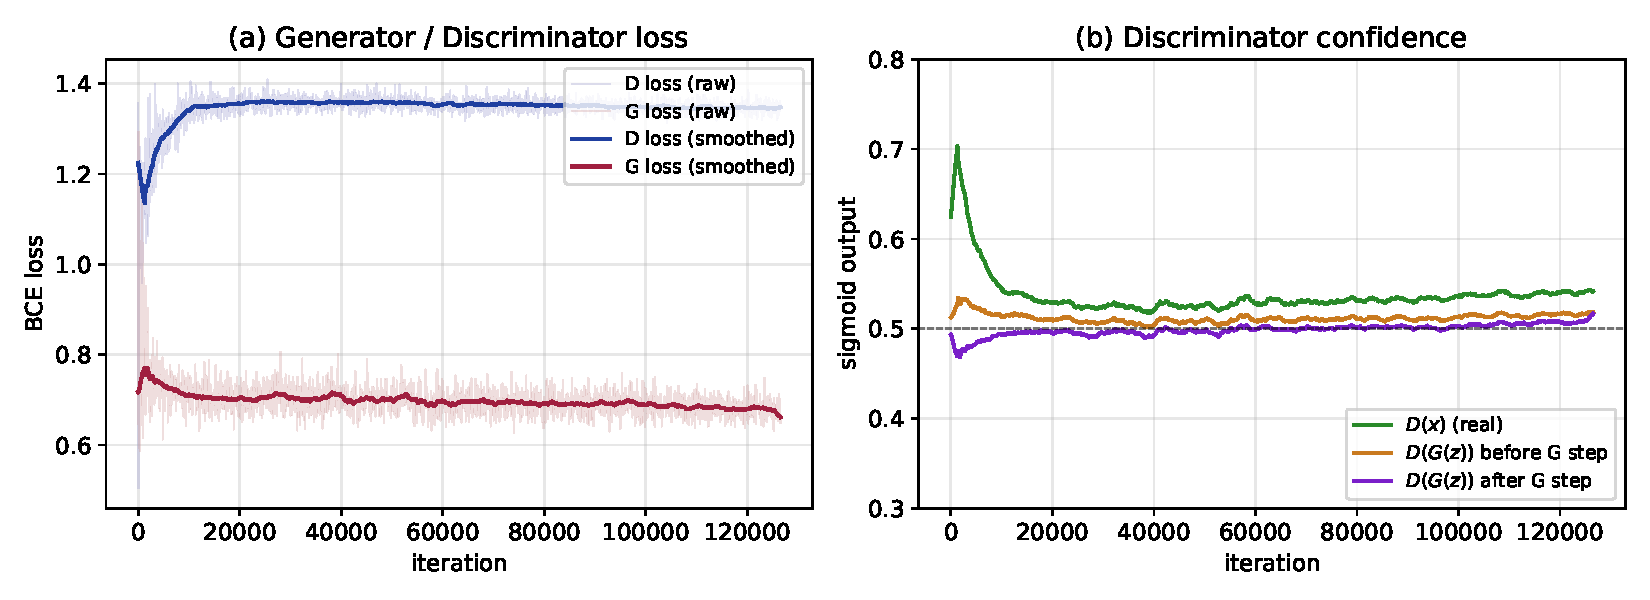
\includegraphics[width=\figwidefull]{figures/dcgan_loss.pdf}
\caption{基线对抗训练动力学。左：生成器与判别器的二分类交叉熵损失，
细线为原始值，粗线为窗口长度 51 的滑动平均。
右：判别器对真实样本与生成样本的概率输出，
理想博弈应在 0.5 附近振荡。}
\label{fig:dcgan-loss}
\end{figure}

\subsection{样本质量随训练步数的演化}
图~\ref{fig:dcgan-prog} 展示了在固定噪声下生成结果随训练步数的演化。
从初始的色块状噪声开始，约 $5\times 10^3$ 步后样本中已经
浮现出粗略的脸部轮廓与肤色块；至 $5\times 10^4$ 步以后
头发、五官位置与皮肤纹理基本稳定，
并在剩余训练中持续锐化高频细节。
固定噪声轨迹中未观察到样本同质化或局部反复跳变，
说明模型未发生明显的模式崩溃。

\begin{figure}[H]
\centering
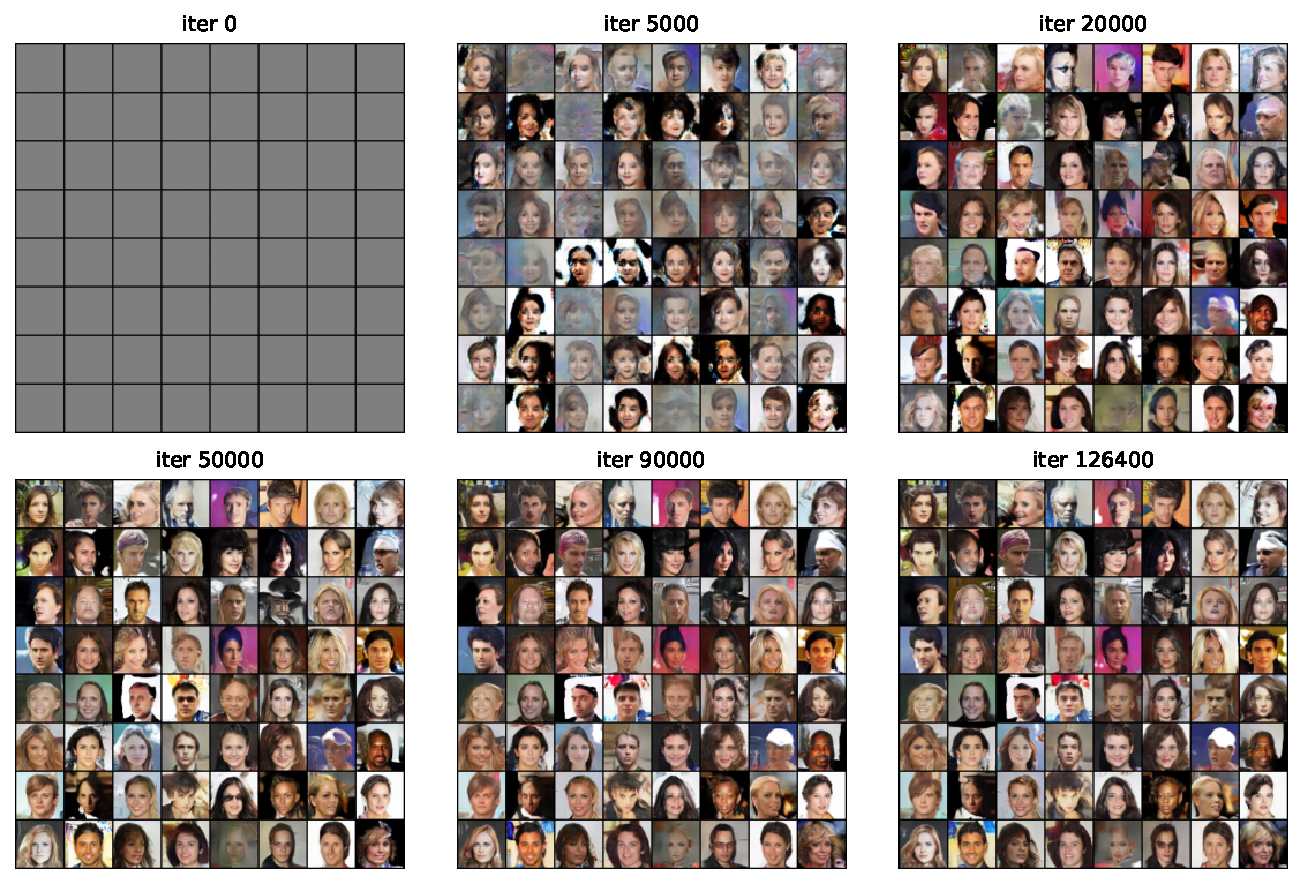
\includegraphics[width=\figwidefull]{figures/dcgan_progression.pdf}
\caption{固定噪声下生成器样本随训练步数的演化，
每张子图为同一噪声批次的网格化输出。}
\label{fig:dcgan-prog}
\end{figure}

\subsection{潜空间插值}
我们在两个独立采样的噪声点之间分别以线性插值与球面插值生成 $10$ 帧。
两条路径的端点完全相同，但中间帧呈现出明显差异：
线性路径中段样本相对模糊，与中段范数收缩造成的「先验偏离」相吻合；
球面路径中段保持原有先验范数，样本锐度与端点保持一致。
两条路径上的姿态、肤色、性别属性均呈现单调的连续过渡，
未观察到突变或重影，说明生成器在采样邻域内学到的是一个连续的人脸流形。

\subsection{定量评估}
对滑动平均生成器各采样 $10^4$ 张样本，
并从真实数据集按相同预处理保存等量的图像，
在统一脚本下同时计算 Fr\'echet Inception Distance 与 Inception Score。
其中，FID 用于衡量生成样本与真实样本在 Inception 特征空间中的分布距离，
数值越低说明生成分布越接近真实分布；Inception Score 则同时刻画样本的清晰度与多样性，
数值越高通常表示生成质量越好。考虑到 Inception Score 对采样划分存在一定波动，
我们同时报告均值与标准差。

基线模型的定量评估结果如表~\ref{tab:baseline-eval} 所示。
在 $64\times 64$ 分辨率下，模型取得了 FID 为 15.74847、Inception Score 为
2.609323 $\pm$ 0.05265605 的结果。
这说明基线模型已经能够生成具有一定清晰度与多样性的脸部样本，
但与高分辨率风格化生成器在样本逼真度与细节表现上的上限相比，
仍然存在明显差距，这也是后续引入进阶分支的主要动机之一。

\begin{table}[H]
\centering
\caption{基线模型的定量评估结果。}
\label{tab:baseline-eval}
\small
\begin{tabular}{lc}
\toprule
指标 & 数值 \\
\midrule
Fr\'echet Inception Distance $\downarrow$ & 15.74847 \\
Inception Score $\uparrow$ & $2.609323 \pm 0.05265605$ \\
\bottomrule
\end{tabular}
\end{table}

\subsection{进阶分支：分层潜空间映射器训练}
对十条文本描述各独立训练一个分层潜空间映射器，
单次训练约 $1.5$ 小时。
图~\ref{fig:mapper-loss} 把十次训练的总损失与 CLIP 损失曲线
叠加显示。可以观察到三个共性现象：
其一，所有训练在约 $5\times 10^3$ 步内进入相对平台期；
其二，进入平台后总损失基本由 CLIP 项主导，
$\ell_2$ 与身份项贡献相对稳定；
其三，全部训练过程未观察到损失反弹或剧烈振荡，
说明本文采用的损失权重与学习率组合在不同语义难度的描述上
具有一致的稳定性。

\begin{figure}[H]
\centering
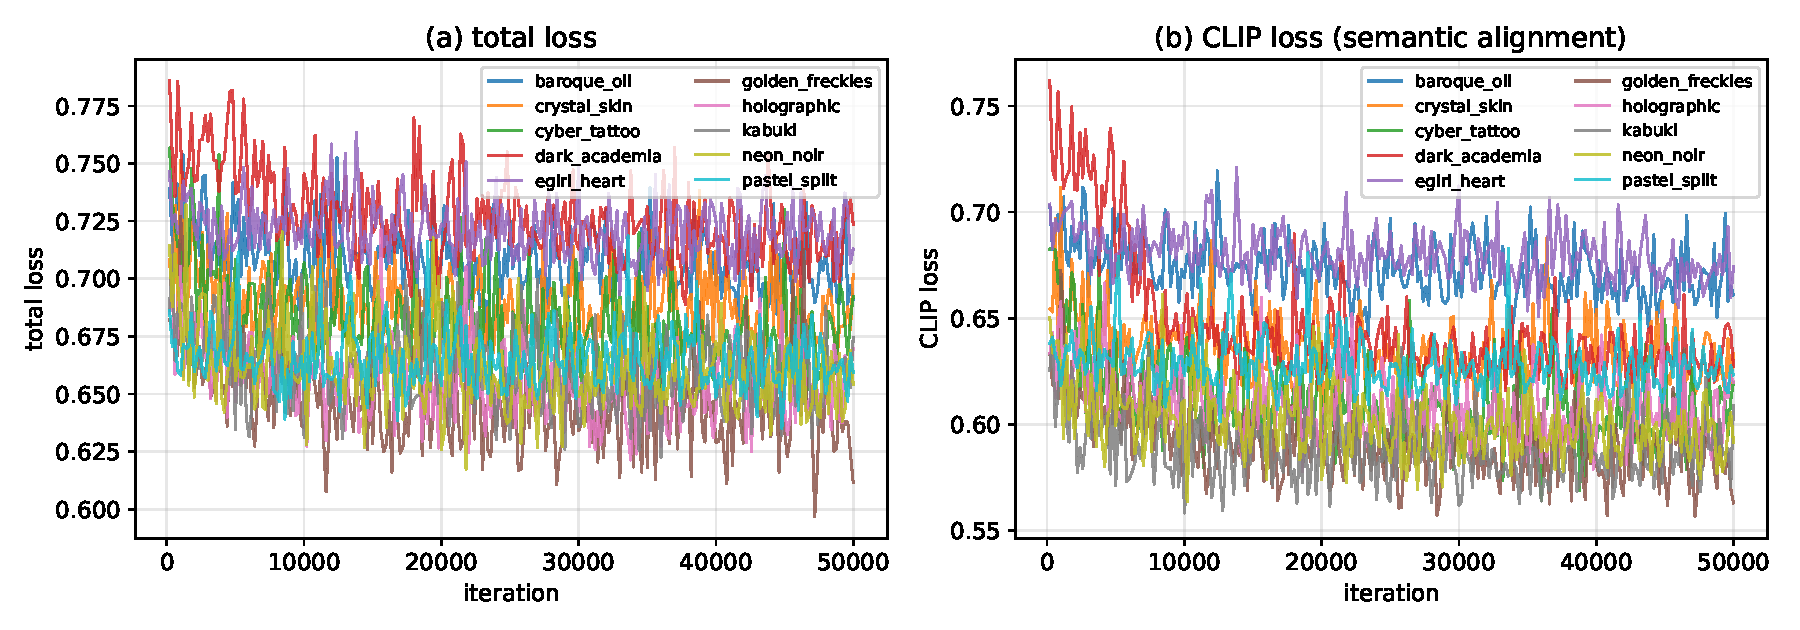
\includegraphics[width=\figwidefull]{figures/mapper_loss_overlay.pdf}
\caption{十个分层潜空间映射器在 $5\times 10^4$ 步训练中的损失曲线。
左：总损失。右：CLIP 语义损失。}
\label{fig:mapper-loss}
\end{figure}

\paragraph{终态损失项之间的权衡}
图~\ref{fig:mapper-final} 与表~\ref{tab:mapper-final} 给出了
每个映射器在最后约 $2\times 10^3$ 步上各损失项的均值。
不同文本描述在三轴上呈现出明显不同的取舍模式：
偏向局部纹理修饰且贴近自然人脸流形的描述
（如金色雀斑、霓虹噪点、歌舞伎妆）取得了最低的 CLIP 损失，
说明骨干生成器原本就具备覆盖此类视觉概念的潜空间方向；
而需要在面部叠加非自然元素的描述（如心形脸贴纸）
则呈现明显较高的 CLIP 损失，对应较弱的语义达成度。
身份损失方面，深色学院风格几乎是唯一明显牺牲身份保真度的描述，
其原因在于该风格倾向于把人物头发、服饰与光照同步推向一个
高度风格化的状态，导致身份特征被相应改写；
$\ell_2$ 位移最大者为发光赛博纹身一类，
反映出在面部贴附复杂结构所需的潜空间位移更大。
整体而言三轴之间的权衡与已有研究中的观察一致，
即语义达成、身份保真与潜空间位移三者难以同时极小。

\begin{figure}[H]
\centering
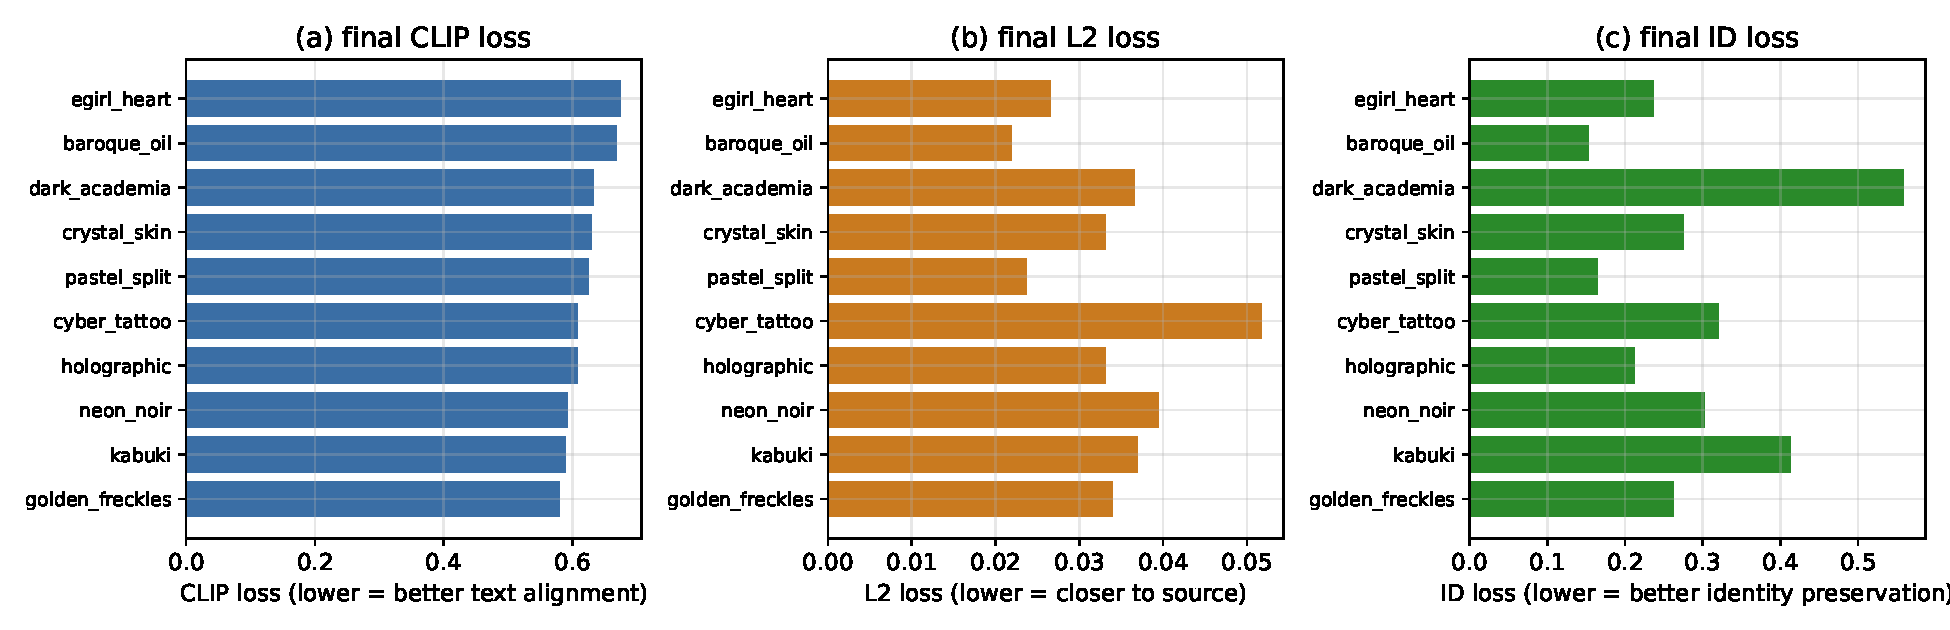
\includegraphics[width=\figwidefull]{figures/mapper_final_metrics.pdf}
\caption{十个映射器训练终态各损失项均值。
按 CLIP 损失从低到高排序。}
\label{fig:mapper-final}
\end{figure}

\begin{table}[H]
\centering
\caption{各映射器训练终态损失项与单次训练时长。}
\label{tab:mapper-final}
\small
\begin{tabular}{lcccc}
\toprule
文本描述 & CLIP $\downarrow$ & $\ell_2$ $\downarrow$ & ID $\downarrow$ & 训练时长 (s) \\
\midrule
golden\_freckles & 0.5805 & 0.0339 & 0.2621 & 5\,488 \\
kabuki           & 0.5901 & 0.0369 & 0.4138 & 5\,469 \\
neon\_noir       & 0.5921 & 0.0394 & 0.3026 & 5\,935 \\
holographic      & 0.6073 & 0.0331 & 0.2122 & 5\,658 \\
cyber\_tattoo    & 0.6082 & 0.0518 & 0.3201 & 5\,535 \\
pastel\_split    & 0.6245 & 0.0237 & 0.1641 & 5\,807 \\
crystal\_skin    & 0.6295 & 0.0331 & 0.2752 & 5\,771 \\
dark\_academia   & 0.6330 & 0.0365 & 0.5587 & 5\,528 \\
baroque\_oil     & 0.6682 & 0.0219 & 0.1534 & 5\,514 \\
egirl\_heart     & 0.6742 & 0.0265 & 0.2368 & 5\,694 \\
\bottomrule
\end{tabular}
\end{table}

\paragraph{编辑结果的定性分析}
图~\ref{fig:mapper-eval} 给出了各文本描述对应映射器在固定评估种子下
的成对编辑网格，每张子图左半为反演得到的源图，
右半为对应的编辑结果；
图~\ref{fig:mapper-pair} 进一步给出训练末期的源图与编辑图对照。
可以观察到，歌舞伎妆、霓虹噪点与全息风格的映射器
显著改变了肤色、化妆与光照色调，但保持了五官位置与人物身份；
金色雀斑映射器在面部均匀添加了细密的金色斑点，
是细分组单独起作用的典型例子；
赛博纹身映射器在脸颊与眉骨附近生成了带有发光质感的图案；
巴洛克油画与深色学院风格则更多改变了整体笔触、色调与服饰；
心形脸贴纸的映射器试图把心形装饰贴附在脸颊上，
但效果相对克制——这与其在 CLIP 损失上落点最高一致，
反映出贴纸类元素本身偏离自然人脸流形，
仅靠潜空间位移难以完全实现。

\begin{figure}[H]
\centering
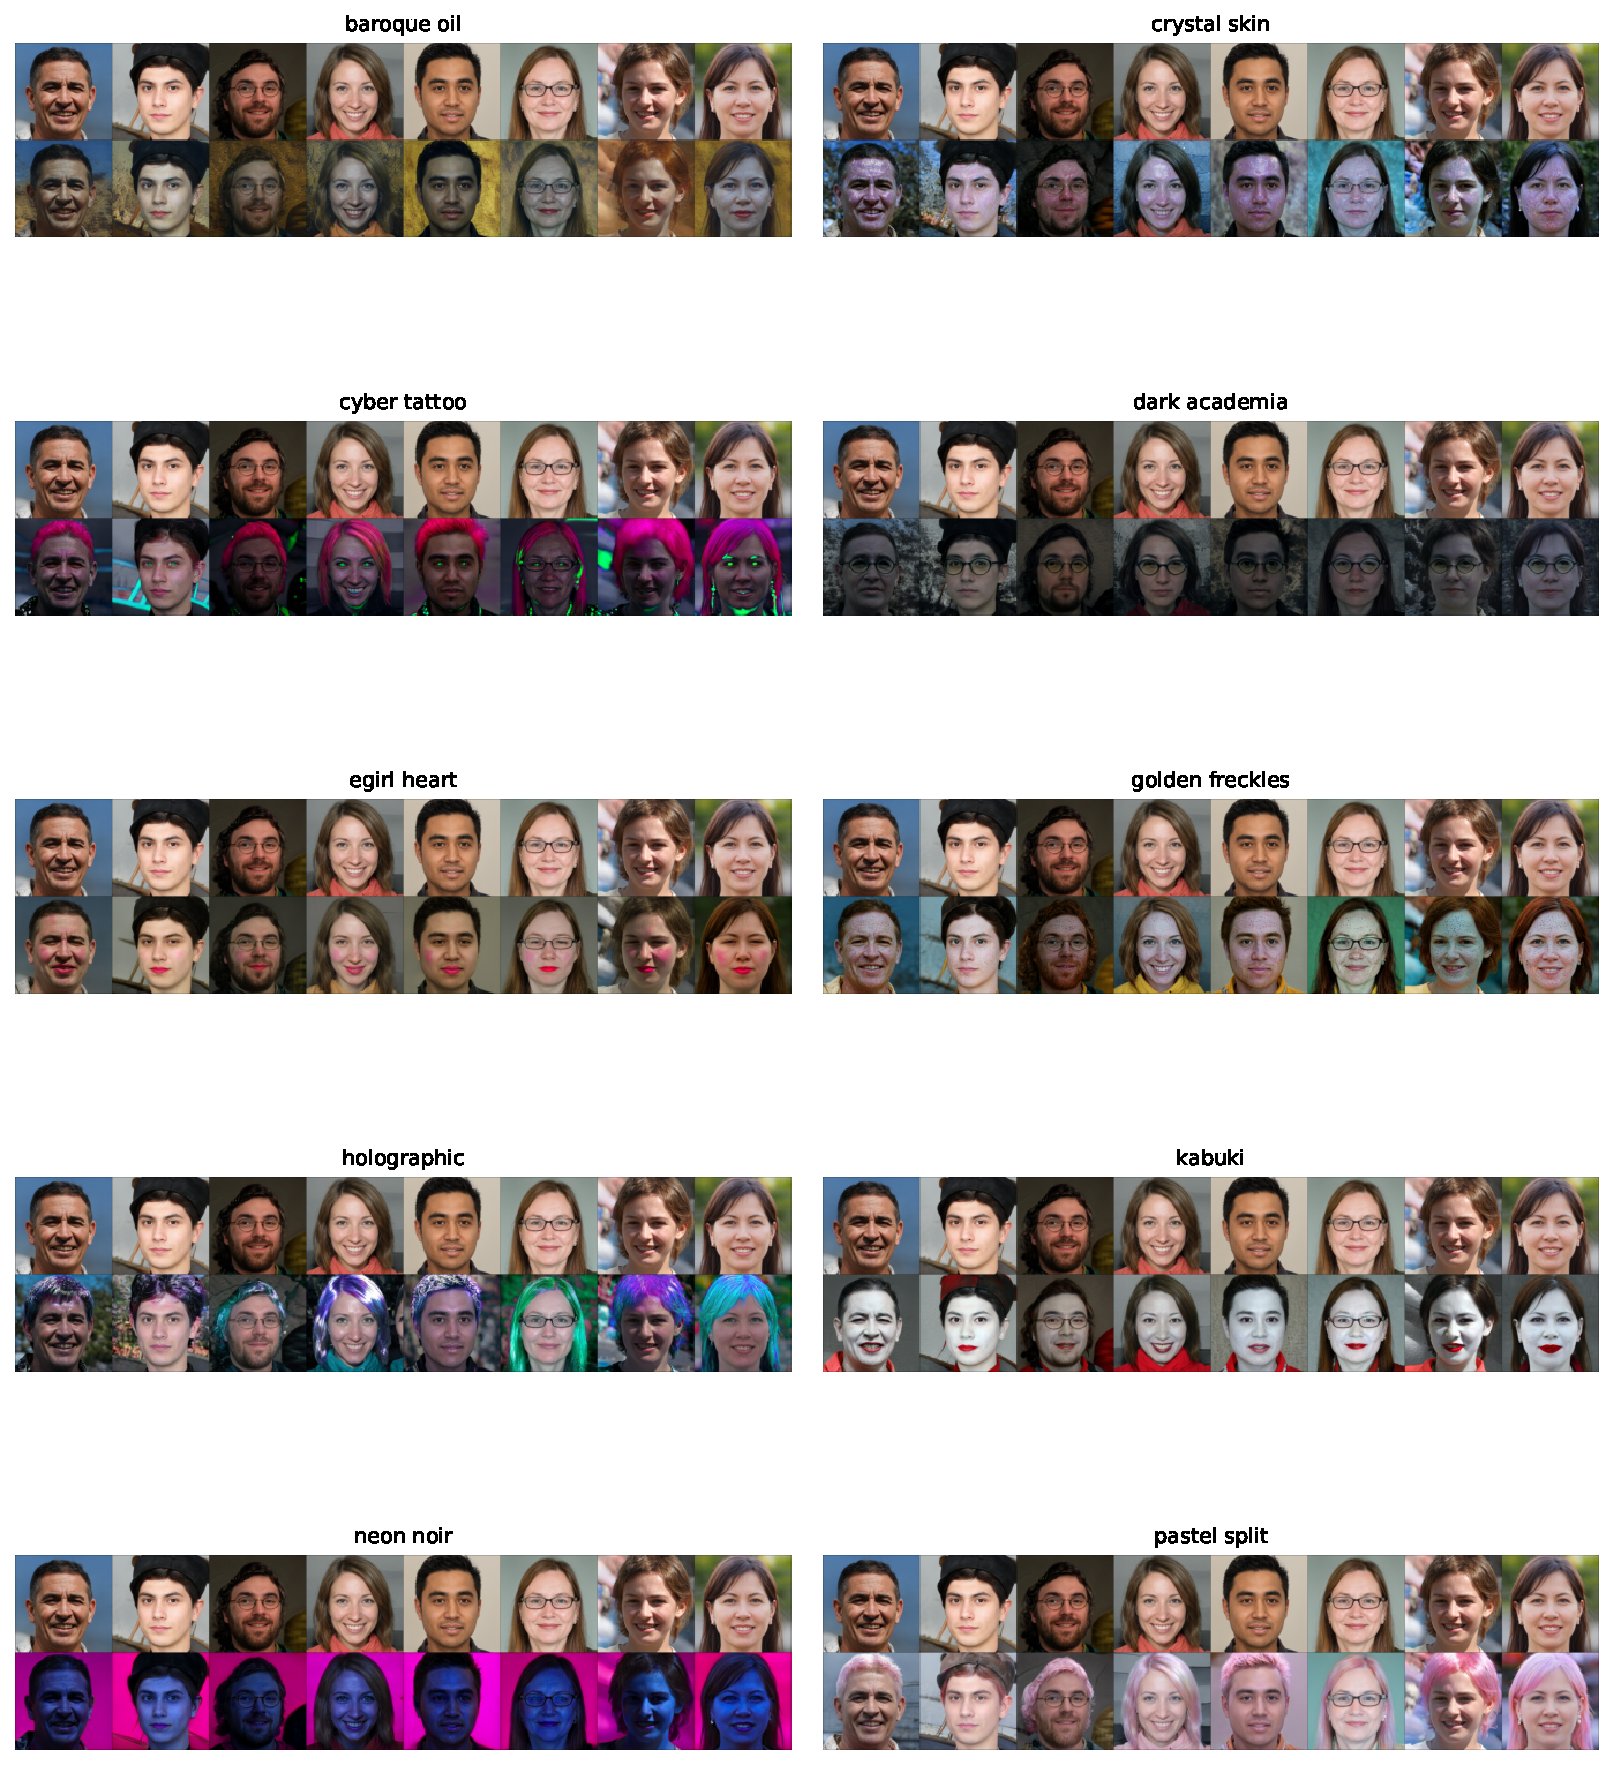
\includegraphics[width=\figwidefull]{figures/mapper_eval_grids.pdf}
\caption{各文本描述对应映射器在固定评估种子下的编辑网格。
每张子图左半为源图、右半为编辑后样本。}
\label{fig:mapper-eval}
\end{figure}

\begin{figure}[H]
\centering
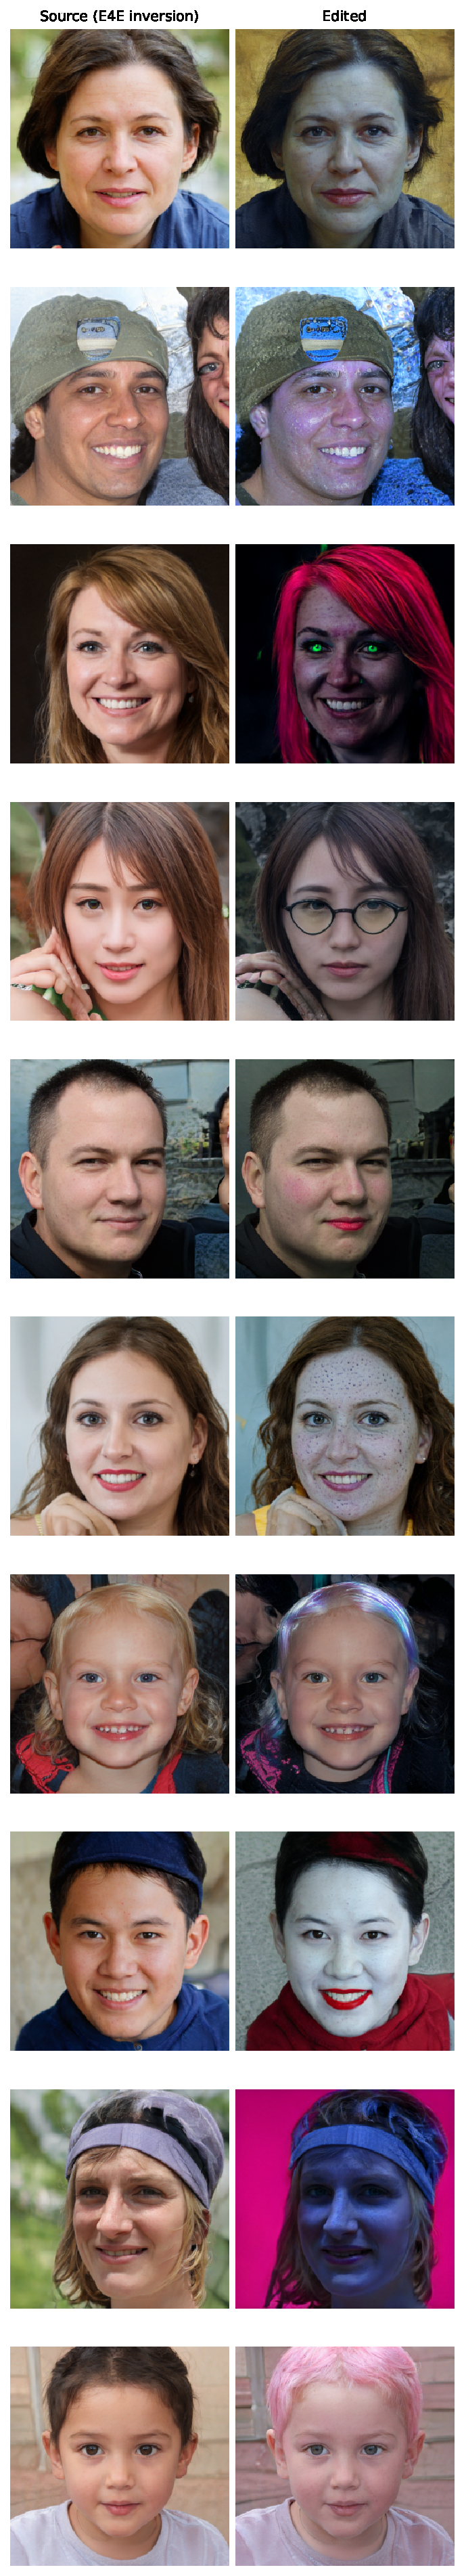
\includegraphics[width=\figwidetall]{figures/mapper_qualitative.pdf}
\caption{训练末期源图与编辑图对照，
每个映射器一行，左列为源图、右列为编辑后。}
\label{fig:mapper-pair}
\end{figure}

%=================================================================
\section{讨论}
%=================================================================

\subsection{两条路径的对比}
基线路径以从零训练为代价，提供了一个完整的对抗训练实验环境，
便于观察损失动力学、样本演化以及缓解模式崩溃所采用的工程手段
是否真正起作用；其代价是受限的分辨率与网络容量，
在样本细节与语义可控性上存在天花板。
进阶路径则以预训练高分辨率风格化生成器为不可训练的骨干，
将研究焦点上移至「如何在解耦潜空间中以最小代价注入语义控制」，
得以在不重新训练生成器的前提下获得多种独立的编辑能力。
两条路径并非替代关系，而是从不同侧面回应了人头图像生成中
「样本质量」与「可控性」两个核心维度。
表~\ref{tab:compare} 对两条路径在主要维度上的差异进行汇总。

\begin{table}[H]
\centering
\caption{基线与进阶分支的主要差异。}
\label{tab:compare}
\small
\begin{tabular}{lll}
\toprule
& 基线 & 进阶 \\
\midrule
分辨率 & $64\times 64$ & $1024\times 1024$ \\
潜空间 & 100 维各向同性正态先验 & $18\times 512$ 解耦风格空间 \\
是否需要训练生成器 & 是（80 轮） & 否（冻结骨干） \\
是否支持文本条件 & 否 & 是（每条描述一个映射器） \\
是否支持真实图像编辑 & 否 & 是（反演 + 映射器） \\
模式崩溃风险 & 较高，需要工程手段缓解 & 极低，由骨干稳定性继承 \\
\bottomrule
\end{tabular}
\end{table}

\subsection{对模式崩溃的实证观察}
本文为缓解模式崩溃所采用的若干工程手段，在最终训练曲线与
固定噪声样本演化中均得到了正向验证。
谱归一化与判别器输入退火噪声共同压低了判别器的「峰值能力」，
平滑标签进一步避免了真假样本概率被推到极端值；
滑动平均生成器使得用于评估和插值的权重更接近真实最优解的
邻域均值，从而显著缓解了单步振荡引起的视觉抖动；
固定噪声下的可视化轨迹则提供了一个低成本的崩溃探针，
便于在训练早期发现样本同质化趋势。

\subsection{语义可达性与文本描述的关系}
进阶分支的实验同时揭示了一个值得注意的现象：
不同文本描述在 CLIP 损失上的最终落点差异较大，
且这种差异并不来自训练超参数，而是来自于文本对应概念
与骨干生成器原始流形之间的对齐程度。
当描述对应的视觉变化主要落在颜色、纹理或局部高频结构时，
通常仅需要细分组的小幅潜空间位移即可达成，
对应的 CLIP 损失明显更低；
而当描述要求贴附或嵌入非自然几何元素时，
仅靠潜空间位移就显得力不从心，CLIP 损失曲线进入更高的平台。
这启示我们，未来若希望在同一框架内更好地处理后一类描述，
可能需要进一步引入显式的空间编辑模块，或在更大的潜空间中训练。

%=================================================================
\section{结论}
%=================================================================
本文沿着「从零训练的卷积对抗网络」与「冻结骨干上的潜空间映射器」
两条路径，完整复现并实验性分析了人头图像生成与编辑的两类典型方案。
在基线侧，我们以谱归一化、滑动平均生成器、平滑标签与
判别器输入退火噪声等手段稳定了对抗训练，
并在固定噪声样本演化、潜空间插值与定量指标三个层面
验证了模型的可用性；
在进阶侧，我们对一组多样化的文本描述各独立训练了一个分层潜空间映射器，
通过 CLIP、身份与潜空间位移三项损失之间的权衡分析揭示了
文本描述的语义可达性与骨干潜空间结构之间的关联。
两条路径在最终生成质量、可控性与训练成本方面形成互补，
共同构成了一个完整的人头图像生成与可控编辑实验框架。

\begin{thebibliography}{9}
\small
\bibitem{goodfellow2014gan} I.~Goodfellow et al.,
\emph{Generative Adversarial Nets}, NeurIPS 2014.
\bibitem{radford2015dcgan} A.~Radford et al.,
\emph{Unsupervised Representation Learning with Deep Convolutional Generative Adversarial Networks}, ICLR 2016.
\bibitem{miyato2018sn} T.~Miyato et al.,
\emph{Spectral Normalization for Generative Adversarial Networks}, ICLR 2018.
\bibitem{karras2019stylegan} T.~Karras et al.,
\emph{A Style-Based Generator Architecture for Generative Adversarial Networks}, CVPR 2019.
\bibitem{karras2020stylegan2} T.~Karras et al.,
\emph{Analyzing and Improving the Image Quality of StyleGAN}, CVPR 2020.
\bibitem{patashnik2021styleclip} O.~Patashnik et al.,
\emph{StyleCLIP: Text-Driven Manipulation of StyleGAN Imagery}, ICCV 2021.
\bibitem{tov2021e4e} O.~Tov et al.,
\emph{Designing an Encoder for StyleGAN Image Manipulation}, SIGGRAPH 2021.
\bibitem{radford2021clip} A.~Radford et al.,
\emph{Learning Transferable Visual Models From Natural Language Supervision}, ICML 2021.
\bibitem{heusel2017fid} M.~Heusel et al.,
\emph{GANs Trained by a Two Time-Scale Update Rule Converge to a Local Nash Equilibrium}, NeurIPS 2017.
\end{thebibliography}

\end{document}
